\section{About X protocol}
The whole application is using the X protocol, we are therefore going
to give a brief presentation of this protocol, for the reader to be able 
to understand the concepts in this paper.
\subsection{Generalities}
The X protocol is a network-transparent protocol for bitmap display. 
It uses a client-server architecture, running the server on the computer 
with the display, and makes the connection with local and remote clients possible. 
It is a binary protocol and can be built on top of any reliable byte stream (eg. TCP).
\subsection{Messages}
The protocol uses four main types of messages to communicate between 
the server and the clients. Those types are
\begin{description}
\item[Requests] A request is the basic way to communicate from the client 
  to the server and can be used either to query for some information or to 
  update the display. Some requests need a reply while other do not. 
  Requests needing a reply can be asyncrhonous or not.
\item[Replies] A reply is the basic way for the server to send back
  information to the client, and is usually used to send information about the server.
\item[Events] Events are generated by the server and sent to the client to notify it of 
  some event in the handled display. Event can be used for graphic events 
  (eg. when a window has been rendered) or for device events (eg. keyboard or mouse event).
\item[Errors] Errors can be generated from the client as well as the server
  for many different reasons. One of the main reason for errors generated 
  from the server side is for access to non available resources.
\end{description}
An overview of how these messages are sent is shown in figure \ref{fig:xcore-overview}.
\begin{figure}[tb]
  \begin{center}
    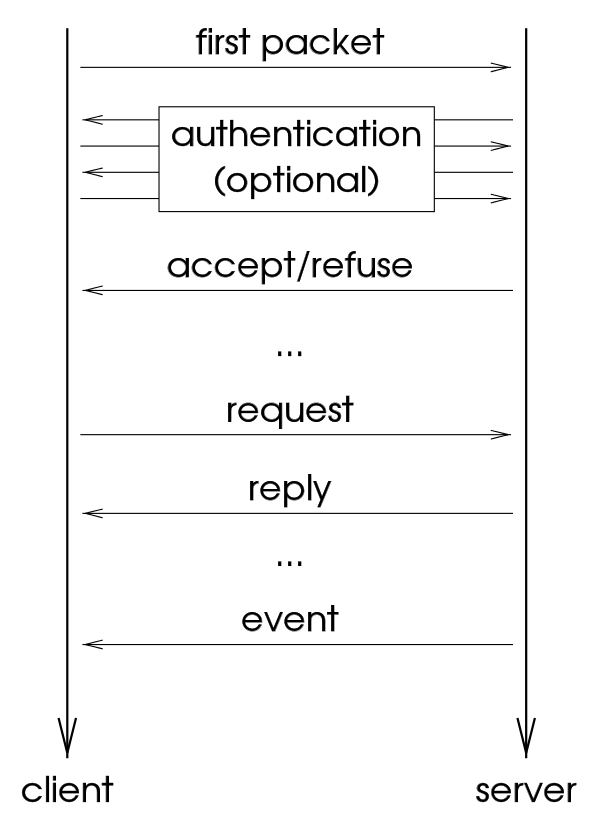
\includegraphics[height=8cm,width=6cm]{../imgs/xcore-overview.png}
    \caption{\label{fig:xcore-overview}Overview of the X protocol}
  \end{center}
\end{figure}
\subsection{Resources}
The protocol uses a number of different resources which we will shortly 
introduce here.
\begin{description}
\item[Drawable] A drawable is an abstract entity used to draw. It can be a window or a pixmap.
\item[Window] There are two types of window: top-level window and subwindows. 
  A top-level window is the main container for an application and 
  usually contains all the other components of the application.
  A subwindow is a window contained in the top-level window of an application 
  and can be used for anything, from the titlebar to a button in the application.
\item[Pixmap] A pixmap is a region used to draw, but on opposite to a window, 
  it is not shown until explicitly requested. The content of a pixmap 
  or part of it can be displayed on a window.
\item[Graphic context] A graphic context is a structure containing basic graphic 
  information to apply to a given request, for example the background and 
  foreground colors, or a transformation to apply to the shape to draw.
\subsection{Short example}
To end up with the presentation of the X protocol, we will here give a
short example of a communication between an X server and an X client.
\end{description}
